\documentclass[a4paper]{article}
\usepackage{graphicx}
\usepackage{geometry}
\usepackage{calc}
\usepackage[percent]{overpic}
\usepackage[medium]{HindMadurai}
\usepackage[T1]{fontenc}
\usepackage{tikz}
\usepackage{multicol}
\usepackage{enumitem}
\usepackage{xcolor}

% \renewcommand\familydefault{\sfdefault}

\newlength{\picmargin}
\setlength{\picmargin}{15pt}

\newlength{\picwidth}
\setlength{\picwidth}{\paperwidth - 2\picmargin}

\geometry{
    top=\picmargin,
    bottom=\picmargin,
    left=\picmargin,
    textwidth=\picwidth
}

\newcommand{\recipeTitle}[1]{
  \vspace{0.2cm}
  \parbox{\picwidth}{
    \centering
    \LARGE{\textbf{#1}}
  }
}

\newcommand{\recipeDescription}[1]{
  \vspace{0.2cm}
  \parbox{\picwidth}{
    \centering
    \large
    {#1}
  }
}

\newcommand{\ingredient}[1]{
  \item[]{#1}\\
}

\newcommand{\prep}[1]{
  \textbf{Prep:} {#1}\\
}

\newcommand{\cooking}[1]{
  \textbf{Cook:} {#1}\\
}

\newcommand{\hide}[1]
{}

\newenvironment{steps}
{%
  \begin{enumerate}[leftmargin=0.3cm]
}
{%
  \end{enumerate}
}

\newenvironment{ingredients}
{%
  \vspace{9pt}
  \begin{itemize}[nosep, itemsep=2pt, leftmargin=3pt]
}
{%
  \end{itemize}
}

\definecolor{Pagebackground}{HTML}
{ffffff} %<{type: "reference", id: "backgroundColor"}>
\pagecolor{Pagebackground}

\definecolor{captionColor}{HTML}
{000000} %<{type: "reference", id: "imageCaptionColor"}>

\definecolor{textColor}{HTML}
{000000} %<{type: "reference", id: "textColor"}>

\begin{document}
\pagestyle{empty}
%<{"type": "group", "description": "Recipe image"}
\hspace{-\picmargin}%
\begin{overpic}[
    width=\picwidth,
    height=0.70\picwidth,
    % grid,
    % tics=10
  ]
    {raspberry-pie-cropped}
  %>
  \put (1,2) {
    \parbox[b]{0.3\picwidth}
    {
      \textcolor{captionColor}{
        \textbf
        %<{
        %   type: "text",
        %   description: "Recipe image caption",
        %   inputValue: "Caption. Say something sweet about this photo or recipe."
        % }>
          {It's like Chipolte's Corn Salsa, but the corn is hot and made fresh}
        %>
      }
    }
  }
\end{overpic}
%>

\color{textColor}

\vspace{0.5cm}
\hspace{-\picmargin}
%<{
%   type: "text",
%   description: "Recipe title",
%   inputValue: "NANA'S RASPBERRY PIE"
% }>
\recipeTitle{Freepolte Corn Salsa}
%>

\vspace{-0.5cm}
\hspace{-\picmargin}
\parbox{\picwidth}{
  \centering
  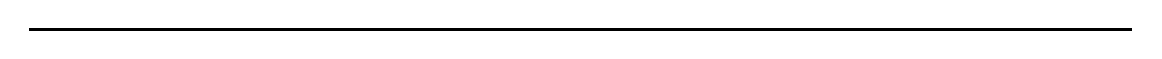
\begin{tikzpicture}
    \draw[very thick] (-7,0) -- (7,0);
  \end{tikzpicture}
}
% \line(1,0){12cm}

\vspace{0.3cm}
\hspace{-\picmargin}
\recipeDescription{My mom doesn't like corn, but she likes this.} 

\begin{multicols}{3}
  \normalsize
  \raggedright
  \textbf{Ingredients}\\
  \begin{ingredients}
      \ingredient{4 ears of fresh sweet corn}
      \ingredient{2 teaspoons of lemon juice}
      \ingredient{2 teaspoons of lime juice}
      \ingredient{1 tablespoon butter}
      \ingredient{1/4 raw red onion}
      \ingredient{2 tablespoons chopped cilantro}
  \end{ingredients}
  %<{"type": "group", "description": "Preparation time"}
    \vspace{0.5cm}
    \prep{15 min}
    \cooking{15 minutes}
    \vspace{0pt}
  %>
  \columnbreak
  \begin{steps}
    %<{"type": "list", "description": "Preparation and cooking steps"}
    \item{De-husk corn}
    \item{Slice corn off of cob and into a medium bowl}
    \item{Pour lemon and lime juice into the bowl}
    \item{Stir occassionaly as it marinades for 20+ minutes for even distribution} 
    \item{Pre-heat pan with olive oil} 
    \item{Add corn and top with butter} 
    \item{Cook over medium heat until it starts to char}
    \item{Remove from heat} 
    \item{Mix in cilantro and red onion} 
    %>
  \end{steps}
\end{multicols}

%<{type: "group", description: "Color settings (optional)"}
\hide{
  %<{type: "color", description: "Page background color", initialColor: "#EEEEEE", id: "backgroundColor", inputValue: "EEEEEE"}>
  %<{type: "color", description: "Image caption color", initialColor: "#000000", id: "imageCaptionColor", inputValue: "000000"}>
  %<{type: "color", description: "Text color", initialColor: "#000000", id: "textColor", inputValue: "000000"}>
}
%>

\end{document}
